\section{Маска хмарності}

Маска хмарності є растровим шаром, у якому %
кожному пікселю відповідає клас поверхні або
атмосферного явища.


Разом з композитами cервіс COAH надає також і маску хмарності.
Вона є масивом із розмірністю, що співпадає з розмірністю самого знімку,
де кожен піксель має значення від 0 до 11 (таб. \ref{tab:cloud-classes}).
Це певний класифікатор, де цифра позначає область знімка, наприклад хмари,
рослинність чи перисті хмари. Відповідно ми можемо одержати інформацію
про кожний піксель композиту, а саме чи є він захмарений чи ні.

\begin{table}[H]
    \begin{center}
        \caption{Класи маски хмарності}
        \label{tab:cloud-classes}
        \begin{tabular}{|p{1.5in} | p{2.3in} |}
            \hline
            \textbf{Значення} & \textbf{Клас} \\
            \hline
            1             &  Немає інформації           \\
            2             &  Дефектні об’єкти           \\
            3             &  Область темних пікселів    \\
            4             &  Тінь хмар                  \\
            5             &  Рослинність                \\
            6             &  Не рослинність             \\
            7             &  Вода                       \\
            8             &  Хмара середньої прозорості \\
            9             &  Не прозорі хмари           \\
            10            &  Прозорі хмари              \\
            11            &  Сніг                       \\
            \hline
        \end{tabular}
    \end{center}
\end{table}

У досліджуваних даних %
використано значення, що позначають чисту
поверхню, хмари, тіні хмар і серпанок.  Для %
побудови бінарної маски хмарними вважалися
класи 2, 3, 8 і 9, а окремо оброблявся клас серпанку.

\section{Недоліки маски хмар від COAH}

На жаль, дані що дає copernicus hub, не є ідеальними, саме це стосується
і маски хмар. Після написання алгоритму було проведено перші його
тестування, результат був неякісним.

Було проведено дослідження чому це відбувається, і виявилось, що не до
всіх знімків класифікатор для маски надається в тому ж самому
розрізнення що і відповідний йому 4 канальний композит. Дана проблема
потребувала вирішення як і для покращення оригінальної маски так і для
алгоритму вилучення хмар.

\begin{figure}[H]
    \centering
    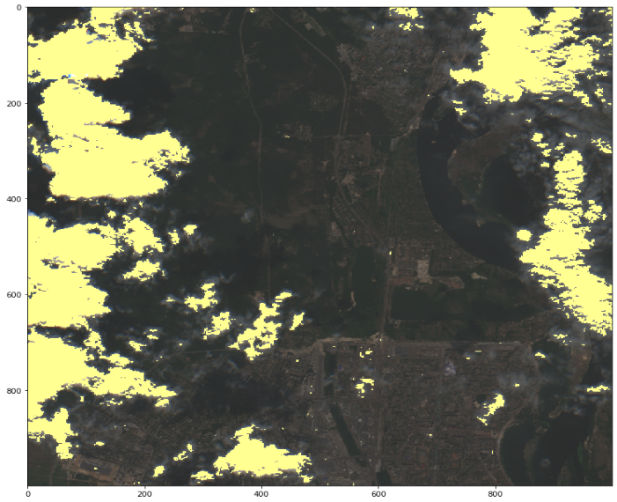
\includegraphics[width=0.7\textwidth]{images/image5}
    \caption{Оригінальна маска хмарності від COAH
        \label{fig:orignal_cloud_mask}
    }
\end{figure}

На завантажених файлах супутникових знімків із розрізненням 10 м
була виявлена маска із розрізненням 20, що й приводило до проблеми
того, що реальні хмари на композиті не покривались класифікатором (рис. \ref{fig:orignal_cloud_mask}).
